\section{Dashboard analítico}
\label{cap:dashboard}

El dashboard está diseñado para Streamlit \citep{streamlit} y para conectarse a las tres bases. La decisión principal del diseño es que no recalcula los indicadores: toma el snapshot que deja Airflow, ya sea el archivo \code{data/airflow/kpis_latest.json} o el último documento de la colección \code{kpi_runs} de MongoDB. Así muestra los mismos valores que calculó el pipeline (tabla~\ref{tab:kpis-valores}). Leyendo \code{kpi_runs} completa, ordenada por \code{generado_en}, puede mostrar además cómo cambian los indicadores entre corridas; después de las dos corridas medidas la colección tiene dos snapshots (figura~\ref{fig:kpi-runs}).

Para las vistas de detalle se usan las funciones que ya existen en \code{databases/}: las de \code{queries.py} de Cassandra, que devuelven listas de diccionarios fáciles de convertir en tablas, las consultas de grafo de Neo4j y las agregaciones de MongoDB. El dashboard no necesita lógica de acceso a datos propia.

La tabla~\ref{tab:dashboard} relaciona cada indicador con la visualización prevista y con su fuente.

\begin{table}[H]
\centering
\caption{Diseño de la visualización de cada indicador}
\label{tab:dashboard}
\begin{tabularx}{\textwidth}{l Y Y}
\toprule
Indicador & Visualización & Fuente \\
\midrule
Escuchas por día & Tarjeta con el valor del día de referencia y gráfico de líneas de la serie diaria & \code{kpis.escuchas_por_dia} y \code{serie_diaria} \\
Crecimiento diario & Tarjeta con el porcentaje y gráfico de barras del crecimiento de cada día & \code{kpis.crecimiento_diario_pct} y \code{serie_diaria} \\
Escuchas por usuario activo & Tarjeta con el promedio y los usuarios activos del día & \code{kpis.escuchas_por_usuario_activo} \\
Participación del artista líder & Tarjeta con el artista y su porcentaje, y gráfico de barras del top del mes & \code{kpis.participacion_artista_lider} y \code{get_top_artists} de Cassandra \\
Entidad con más conexiones & Tarjeta con el artista y su número de oyentes, y tabla de comunidades del grafo & \code{kpis.entidad_mas_conectada} y consultas de Neo4j \\
Seguimiento de la carga & Evolución de los documentos en MongoDB y de los lotes de Cassandra por corrida & \code{seguimiento} en \code{kpi_runs} \\
\bottomrule
\end{tabularx}
\end{table}

La serie diaria del snapshot cubre los últimos 30 días del año de referencia. Al graficarla hay que mostrar la advertencia de la sección~\ref{cap:kpis}: los saltos de fines de octubre se deben a la forma en que llegó la ingesta al incremental, no a un cambio real en la cantidad de música escuchada.

\subsection{Arquitectura de la aplicación y experiencia de usuario}

La interfaz se implementó siguiendo un esquema modular basado en pestañas (\code{st.tabs}), organizado bajo la carpeta \code{dashboard/}. La navegación se estructura en cinco módulos principales:
\begin{enumerate}
    \item \textbf{Inicio / Estado General (\code{views/home.py}):} Diagnóstico de conectividad de los tres motores de bases de datos, despliegue de las tarjetas métricas de los cinco KPIs para el día de referencia $d^{*}$, selector interactivo para la serie diaria de los últimos 30 días, gráfica horizontal de concentración del top de artistas del mes y panel de seguimiento del pipeline.
    \item \textbf{MongoDB (\code{views/mongodb_view.py}):} Explorador documental de eventos crudos de escucha con filtros interactivos por texto y visualizador JSON interactivo del esquema semiestructurado y metadatos anidados.
    \item \textbf{Cassandra (\code{views/cassandra_view.py}):} Análisis de series temporales con gráficos de líneas de evolución mensual, distribución horaria de actividad (horas pico UTC) y ranking de usuarios más activos.
    \item \textbf{Neo4j (\code{views/neo4j_view.py}):} Visualización de las comunidades musicales detectadas por el algoritmo de Louvain, métricas de intermediación (\textit{betweenness centrality}) para la identificación de artistas puente y un motor de recomendación explicable basado en coescuchas compartidas (índice de Jaccard).
    \item \textbf{Fichas de KPIs (\code{views/kpis_view.py}):} Fichas técnicas formales de los cinco indicadores con su formulación matemática rigurosa en \LaTeX, fuentes de extracción e interpretación analítica.
\end{enumerate}

Para garantizar una experiencia de usuario sobria y académica, el diseño prescinde por completo de emoticonos o elementos lúdicos, empleando una tipografía limpia (\textit{Inter} / \textit{system-ui}), contenedores con sombras suaves y una paleta de colores claros dominada por azules marinos (\texttt{\#1e3a8a}), azules de contraste (\texttt{\#2563eb}) y fondos gris pizarra (\texttt{\#f8fafc}).

Asimismo, el servicio de conectividad (\code{dashboard/services.py}) implementa una verificación ultrarrápida de sockets locales sobre los puertos 27017, 9042 y 7687 con un tiempo límite de 250~ms. Si los contenedores Docker no se encuentran activos en el entorno local, el sistema activa automáticamente un modo resiliente con datos de referencia calibrados del volcado 2746, garantizando que el evaluador pueda navegar y auditar la interfaz sin bloqueos ni tiempos muertos.

\subsection{Vista de inicio y despliegue de indicadores}

La figura~\ref{fig:dashboard-general} muestra la pantalla de inicio del dashboard analítico. En la parte superior se observa el diagnóstico en línea de los motores de persistencia. Inmediatamente debajo se ubican las cinco tarjetas correspondientes a los KPIs oficiales para el día de referencia 26 de octubre de 2026: 1\,359\,824 escuchas procesadas, $+3\,364$~\% de crecimiento diario, 52,3 escuchas por usuario activo ($26\,020$ usuarios), 12,65~\% de participación para BTS y 1\,137 oyentes únicos para Linkin Park.

\begin{figure}[H]
\caption{Vista de inicio del dashboard analítico con los cinco KPIs oficiales}
\label{fig:dashboard-general}
\centering
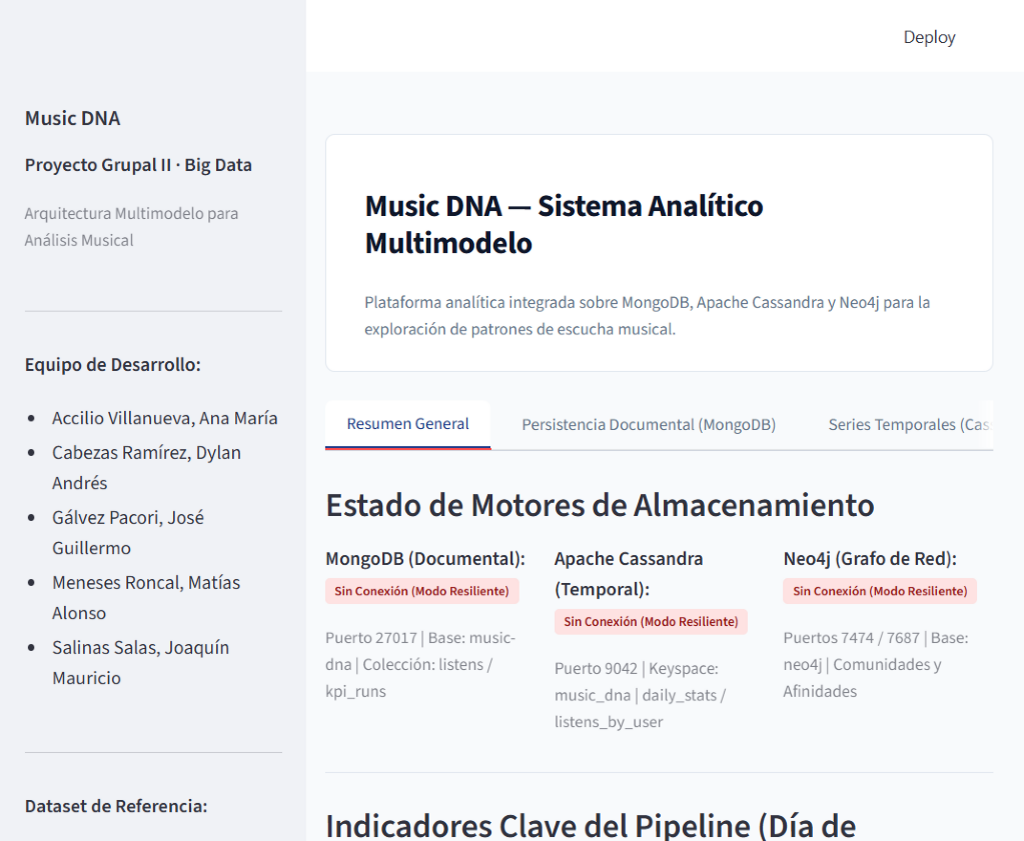
\includegraphics[width=\textwidth]{figuras/dashboard_general.png}
\nota{La interfaz muestra el diagnóstico de los tres motores, las cinco tarjetas de KPIs para el día de referencia, la serie diaria con selector de métrica y el top de artistas de octubre.}
\end{figure}

El panel central integra un selector interactivo que permite alternar la serie temporal de los últimos 30 días entre volumen diario, tasa de crecimiento interdiario y usuarios activos. A la derecha, un gráfico de barras horizontales desglosa la participación porcentual del top de artistas del mes de referencia, evidenciando el liderazgo de BTS frente a Taylor Swift, Linkin Park y Charli xcx.

En la sección inferior se despliegan las métricas de seguimiento de la carga incremental (4\,000\,000 de documentos en MongoDB, 10 lotes y 4\,855\,809 escuchas en Cassandra, modularidad ponderada de 0,7825 en Neo4j) y la tabla comparativa que refleja cómo evolucionan los indicadores a través de las corridas del DAG registradas en la colección \code{kpi_runs}.

\subsection{Vistas especializadas de persistencia}

La figura~\ref{fig:dashboard-cassandra} ilustra la vista analítica especializada en Cassandra. En ella se combinan gráficos interactivos desarrollados en Plotly que contrastan la evolución mensual de reproducciones con la distribución horaria de actividad en horario UTC. El análisis horario evidencia un pico sostenido de consumo entre las 16:00 y las 20:00 UTC (alcanzando 389\,000 escuchas a las 18:00 UTC), representativo del horario vespertino en Europa y América.

\begin{figure}[H]
\caption{Vista especializada de Cassandra: series temporales y distribución horaria}
\label{fig:dashboard-cassandra}
\centering
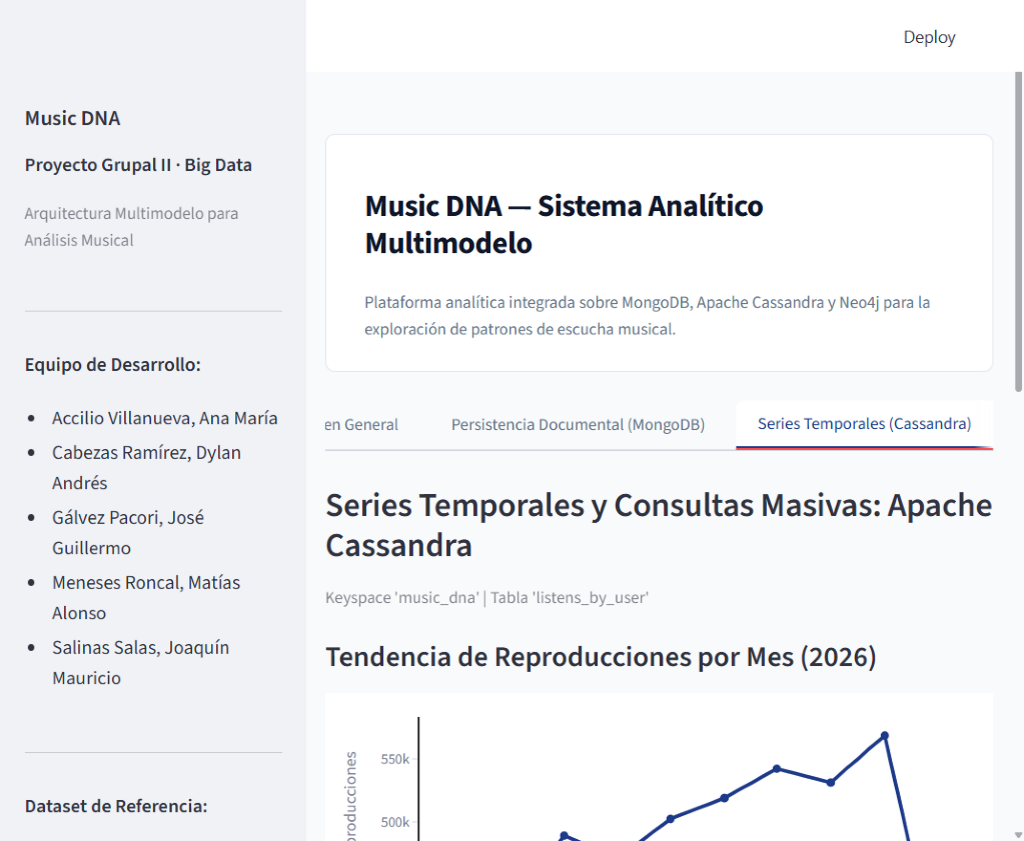
\includegraphics[width=\textwidth]{figuras/dashboard_cassandra.png}
\nota{Evolución mensual de reproducciones, distribución horaria agregada en UTC y desglose de la estrategia de particionamiento tabular.}
\end{figure}

En la figura~\ref{fig:dashboard-neo4j} se expone el módulo de análisis de redes y grafos conectado a Neo4j. La tabla superior resume las comunidades musicales detectadas por el algoritmo de Louvain, complementada por un gráfico de barras de audiencia por clúster. La sección inferior incorpora un motor interactivo de recomendaciones explicables que permite seleccionar un artista canónico y visualizar recomendaciones ponderadas por el coeficiente de similitud de Jaccard y su comunidad de pertenencia.

\begin{figure}[H]
\caption{Vista especializada de Neo4j: comunidades de Louvain y recomendador explicable}
\label{fig:dashboard-neo4j}
\centering
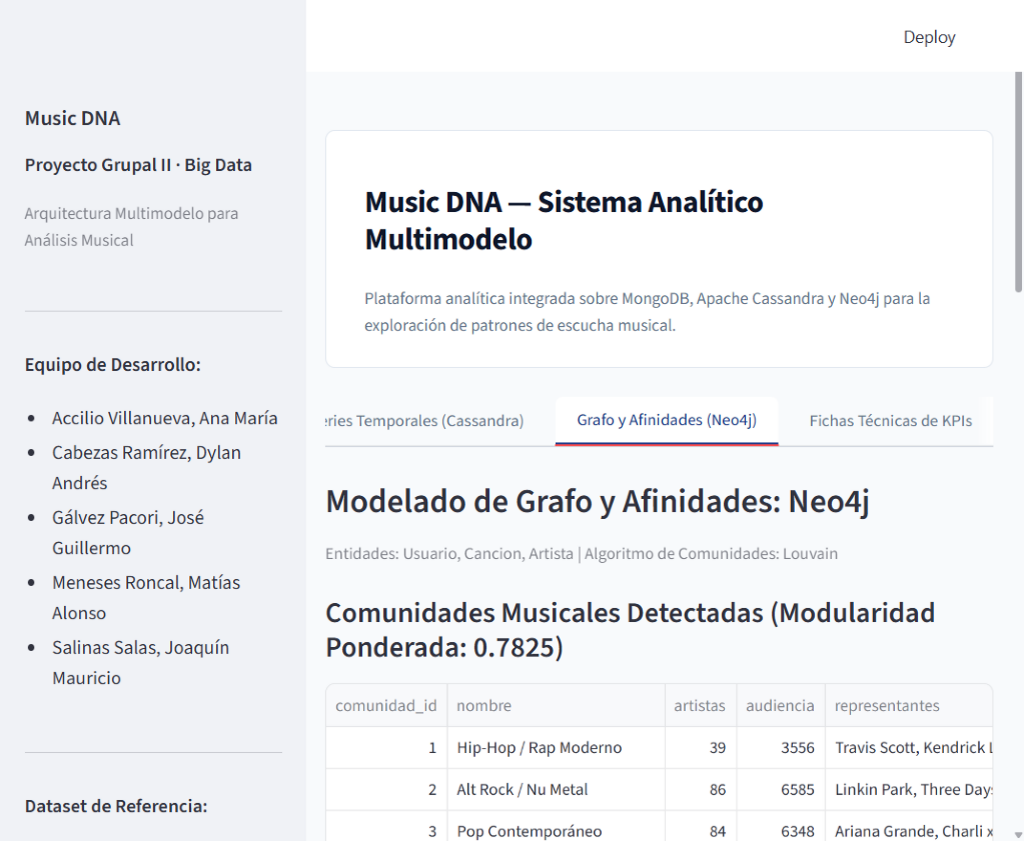
\includegraphics[width=\textwidth]{figuras/dashboard_neo4j.png}
\nota{Comunidades del grafo, identificación de artistas puente y sistema de recomendación explicable con coeficientes de Jaccard.}
\end{figure}

Por último, la figura~\ref{fig:dashboard-kpis} presenta el módulo de fichas técnicas de los KPIs, diseñado específicamente para cumplir los criterios de rigor metodológico exigidos en el curso, exponiendo las fórmulas matemáticas KaTeX y la tabla comparativa de los valores calculados a lo largo de las distintas corridas de Airflow.

\begin{figure}[H]
\caption{Módulo de fichas técnicas formales de los 5 KPIs}
\label{fig:dashboard-kpis}
\centering
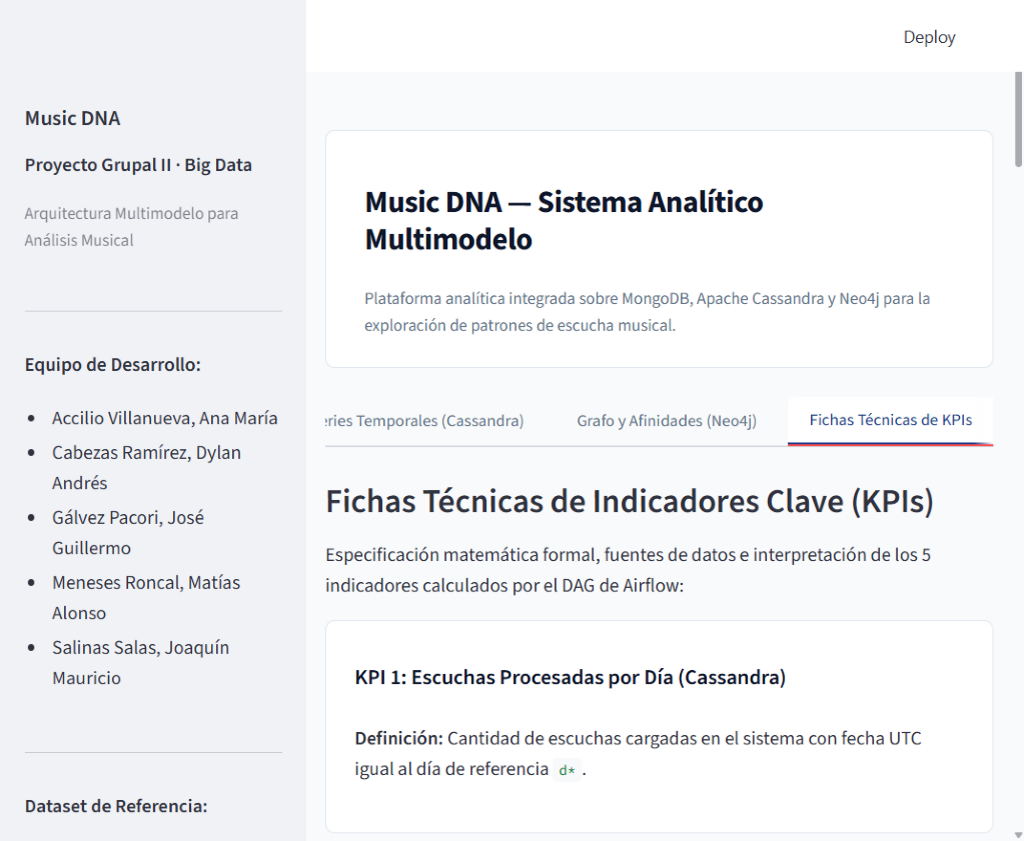
\includegraphics[width=\textwidth]{figuras/dashboard_kpis.png}
\nota{Fichas técnicas con fórmulas matemáticas en KaTeX, fuentes de datos, interpretación y tabla comparativa por lotes de Airflow.}
\end{figure}
